\chapter{A unified language of cellular ABMs}

\epigraph{Before I came here I was confused about this subject. Having listened to your lecture I am
still confused. But on a higher level.}
{\textit{Enrico Fermi}}

\begin{itemize}
    \item theoretical/mathematical treatment of \acp{abm}
    \item characterize overarching concepts between frameworks (simulation concepts)
    \item formulate mathematical notions to capture many (not necessarily all) \acp{abm}
    \item discuss parameter estimation, coarse-graining and pattern formation along these ideas
    \item "Language of \acp{abm}" (important: "A" language, not "the only one")
\end{itemize}

%---------------------------------------------------------------------------------------------------
\section{Theoretical Framework}
\begin{itemize}
    \item use to-be-released paper
\end{itemize}

%---------------------------------------------------------------------------------------------------
\section{Parameter Estimation \& Sensitivity Analysis}
%---------------------------------------------------------------------------------------------------
\section{Coarse-Graining}
\begin{itemize}
    \item bacterial branching
\end{itemize}

%---------------------------------------------------------------------------------------------------
\section{Pattern Formation}

%###################################################################################################
\section{Introduction}
\subsection{Cells as the Fundamental Building Blocks of Nature}
\subsection{Individual-Based Mathematical Treatment}
\subsection{Overarching Principles}

\begin{figure}[H]
    \centering
    \includegraphics[width=\textwidth]{figures/abm-theory/concept-figure.png}
    \caption[Modeling concept figure]{\todo[inline]{explain concept Figure}}
\end{figure}

%###################################################################################################
\newpage
\section{Theoretical Framework}

\begin{itemize}
    \item Start listing example aspects of cellular systems
    \item group aspects in table in (C) Cellular, (CC) Cell-Cell, (EC) Environment-Cell
    \item Concept figure to distinction of these aspect groups
    \item Discuss variations of these aspects on a conceptual level
    \item Discuss underlying assumptions: spatial locality, individual-based behaviour leads to
        collective effects
    \item Discuss how to "throw away" certain parts of this modeling approach (i.e. uniqueness)
\end{itemize}

\begin{table}[h]
    \centering
    \begin{tabular}{cll}
        & \textbf{Modeling Aspect} & \textbf{Examples}\\
        \toprule
        (C) & Mechanics & Spherical, Rod, Rectangular, Hexagonal, Puzlle-shaped\\
        (C) & Intracellular Reactions & Metabolism, Gene-Regulatory Networks\\
        (C) & Cycle & Phases, Division, Death\\
        \midrule
        (CC) & Physical Interaction & Adhesion, Friction, Collisions\\
        (CC) & Contact Reactions & Gap Junctions\\
        \midrule
        (EC) & External Forces & Gravity, Gel Pressure\\
        (EC) & Extracellular Reactions & Diffusion, Fluid Dynamics\\
        \bottomrule
    \end{tabular}
    \caption[Simulation Aspects]{TODO}
\end{table}

%---------------------------------------------------------------------------------------------------
\subsection{The Cellular Space $\CS$}
\label{subsec:cellular-space}
This section aims to construct a space in which individual cells can be represented.
We construct these notions purely from known biological behavioural principles.
By formulating these concepts in abstract mathematical terms, we allow ourselves to cover a wide
variety of \acp{abm}.
It is clear that this approach targets models on the mesoscopic scale such that not every
fundamental effect can be taken into account.

We assume that each individual cell lives in a set $C$ which describes all possible configurations
of this single cell.
We will therefore call this set the "cellular configuration space".
Cellular systems are characterized by the fact that cells are in principle (although in
practice sometimes more difficult) tracable through time and space.
Depending on the cellular representation we might encounter two cells with identical parameters and
properties (eg. position, intracellular concentrations) which are still distinct agents and can not
be interchanged arbitrarily.
This case could occur eg. when representing cellular positions by whole numbers as in a
\ac{ca}.
This point is further made clear when thinking about cellular proliferation as a tree.
Figure~\ref{fig:cell-lineage-break} shows a hypothetical change between two child-cells.
If we would interchange child $c_{12}$ with $c_{21}$, this would mean that two grandchild-cells
$gc_{212}$ and $gc_{221}$ would have different grandparent-cells.

\begin{figure}[h]
    \centering
    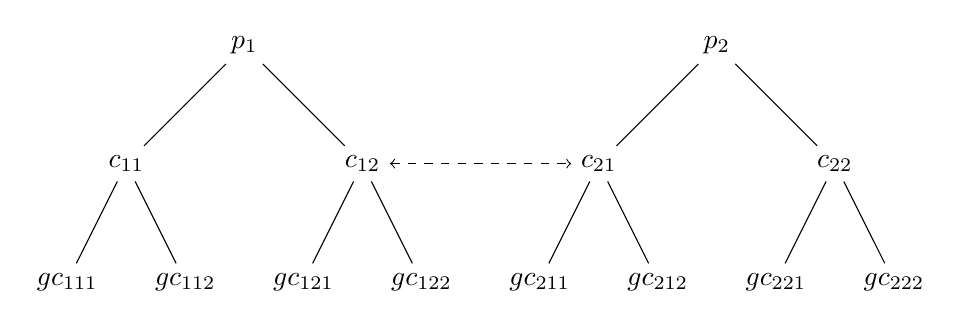
\begin{tikzpicture}[level distance=1.5cm,
            level 1/.style={sibling distance=3cm},
            level 2/.style={sibling distance=1.5cm}
        ]
        \node (p1) {$p_1$}
        child {node (c11) {$c_{11}$}
            child {node (gc111) {$gc_{111}$}}
            child {node (gc112) {$gc_{112}$}}
        }
        child {node (c12) {$c_{12}$}
            child {node (gc121) {$gc_{121}$}}
            child {node (gc122) {$gc_{122}$}}
        };
        \node[] at (6, 0) {$p_2$}
        child {node (c21) {$c_{21}$}
            child {node (gc211) {$gc_{211}$}}
            child {node (gc212) {$gc_{212}$}}
        }
        child {node {$c_{22}$}
            child {node (gc221) {$gc_{221}$}}
            child {node (gc222) {$gc_{222}$}}
        };
        \draw[dashed,<->] (c12) -- (c21);
    \end{tikzpicture}
    \caption[Cell lineage tree]{
        Arbitrary cells can not be interchanged freely since this might introduce incorrect
        configurations into the cell-lineage.
        For example, the two cousin-cells $gc_{212}$ and $gc_{221}$ would have different
        grandparent-cells if $c_{12}$ and $c_{21}$ would be interchanged.
    }
    \label{fig:cell-lineage-break}
\end{figure}

This exemplifies the need to assign unique identifiers for cells to correctly trace their lineage.
We call the set of all identifiers $J$ and only consider cells as a combination of an element
$c\in C$ with an identifier $\iota\in I$.
Thus a cell is an element of the product $J\times C$.
The explicit representation of $J$ can depend on the respective system in question.
To allow for processes such as cell-division and death we additionally must be able to treat a
variable number of cells throughout the evolution of the dynamical system.
The evolution function of our dynamical system will map cellular states onto each other, thus
acting on the cellular space $\CS$.
As can be seen from Figure~\ref{fig:cell-lineage-break}, division of cells introduces two new
identifiers for two new cells and consumes the previously existing cell.
Cell-death removes cells.
Newly inserted cells may not obtain previously used identifiers since this would again interfere
with cell lineage.
This means, we need to keep track of all identifiers $\iota\in I_p$ which have been used in the
past.

\begin{definition}[Cellular State]
    \label{def:cellular-state}
    Let $I$ be a set of identifiers and $C$ be the set describing cellular agents.
    We call a set of cells $(I_p,M)\in Pot(I)\times Pot(I\times C)$ a cellular state if
    \begin{enumerate}
        \item Every cell has a unique identifer $\#\pi_1(M)=\#M$.
        \item Identifiers have not been used previously $I_p\cap\pi_1(M)=\emptyset$
    \end{enumerate}
    where $\pi$ is the projection on the first component.
    The set $I_p$ contains identifiers which have been used previously.
\end{definition}

\begin{definition}[Cellular Space]
    \label{def:cellular-space}
    The cellular space $\CS(I, C)$ of an index set $I$ and cellular configuration space $C$
    is given by
    \begin{equation}
        \CS(I,C) = \{M\in Pot(I)\times Pot(I\times C) | M \text{ is cellular state }\}.
    \end{equation}
    We may choose the simplified notation $\CS = \CS(I, C)$ where the context is
    clear.
    We write $c_\iota:=(\iota,c)\in M$ where $(I_p,M)\in\CS$ despite the non-exhaustiveness
    of the index $\iota$ in a single cellular state.
\end{definition}

Cell division~\cite{bhlitem268752} is a process during which a cell transforms either via binary
(or multiple) fission~\cite{Biov2014} or mitosis~\cite{Ilowiecki1981,von1835resp} and
meiosis~\todo{CITATION} into separate
daughter cells.
To describe cell division, the dynamics behind this transition needs to be taken into account.
We will discuss this in the chapter~\ref{section:dynamics}.
In our agent-based approach, the end of this transition removes the old cell and inserts the new
daughter cells.

\begin{definition}[Single Cell Division]
    \label{definition:cell-division-single}
    We call a map $\gamma:C\rightarrow \cup_{n\geq 2}C^n$ a single division function and
    $\Upsilon:\{\gamma:C\rightarrow \cup_{n\geq 2}C^n\}\times I\times\CS\rightarrow\CS$ a
    single division operator if for any initial state $(I_p,M)\in\CS$ with $d_i\in M$ and
    final state $(J_p,N)=\Upsilon(\eta,i,(I_p,M))$
    \begin{enumerate}
        \item (Removal) Exactly one cell is removed $M\backslash N=\{d_i\}$
        \item (Insertion) At least two new cells are created:
            $N\backslash M=\{c_\iota,\tilde{c}_{\tilde{\iota},\dots}\}$
        \item (Tracking) We carry forward all old identifiers and the removed one:
            $J_p=I_p\cup\{i\}$
        \item (Uniqueness) New cells have new identifiers: $\iota,\tilde{\iota},\dots\notin J_p$.
    \end{enumerate}
    In the case when $i\notin\pi_1(M)$, we require $\Upsilon(\eta,i,(I_p,M))=(I_p,M)$.
    The last two conditions are to be thought of as one in order to guarantee uniqueness for each
    cell over the course of the total time of our system.
\end{definition}

\begin{definition}[Cell Division]
    \label{definition:cell-division-function}
    A division function $\gamma$ is the concatenation of single division functions
    $\{\gamma_i,i\in I\}$.
    We require that the overall effect is independent of the order of their individual applications,
    ie.
    \begin{equation}
        \prod\limits_{i_j\in I}\gamma_{i_j} = \prod\limits_{i\in I}\gamma_i
    \end{equation}
    where the product is with respect to the concatenation of maps.
\end{definition}

It is important to note that while this definition seems cumbersome in the first place, it is
essential in upkeeping a valid cellular state.
From an application standpoint, it is desirable to only specify the division map $\gamma$ and have
$\Upsilon$ be defined by the underlying modeling framework.

Any single-cell division function is only executed once the division process is completed and the
two new daughter cells can be identified.
To indicate the end of the division process a division criterion is used.

\begin{definition}[Cell Division Criterion]
    \label{definition:cell-division-criterion}
    A division criterion is a map $\bar{\gamma}:\mathscr{C} \rightarrow \{0,1\}$ which
    determines if the
    single division function~\ref{definition:cell-division-single} for the particular cell $c$ is
    realized.
\end{definition}

Another important process is that of cell death which is similarly as cell-division not instantanous
but occurs over a period of time.
Death schemes are categoritzed into programmed cell-death, also known as apoptosis~\cite{Kerr1965}
and necrosis~\cite{Gerschenson2001} which occurrs due to damage from external effects.
In principle, these processes take time in order to commence and the cell may interact with its
environment (ie. through secretion) during this stage.
Such transitions can be described by \todo{fill this} and will be discussed in
chapter~\ref{section:dynamics}.
Once the process of dying is over, the cell is removed.

\begin{definition}[Cell Removal]
    \label{definition:cell-death}
    % We call a map $\zeta:I_p\rightarrow \text{Pot}(I_p)$ a death-function
    Any cell-death removes a particular index $\iota\in I_p$.
    Thus the combination of many cell-daths is a mapping $\zeta:I_p\rightarrow \text{Pot}(I_p)$
    where $\text{Pot}(I_p)$ is the power set of $I_p$.

    \todo{
        - apoptosis
        - necrosis
        - removal
    }
\end{definition}

\begin{lemma}[Cell Lineage]
    \label{lemma:cell-lineage}
    Given an initial state $(I_p,M)\in\CS$, an arbitrary combination of applications of
    division and death functions creates a forest.
\end{lemma}
\begin{proof}
    We proof this statement via induction. For $n=0$ we are presented with a cellular state
    $M\in\CS$ which consists of cells $\{c_\iota\in M\}$.
    We interpret each cell as root of a new tree.
    In the induction step $n\rightarrow n+1$, we may assume that $G=(C,E)$ is a tree with
    cells as vertices.
    Any application of a division function $\Upsilon(\gamma, \dot)$ consumes a cell $c_{\iota_0}$
    and produces new cells $\{c_{\iota_1},\dots,c_{\iota_n}\}$.
    We thus insert the new cells as additional vertices with the edges
    $\{c_{\iota_0},c_{\iota_1}\},\dots,\{c_{\iota_0},c_{\iota_n}\}$.
    From the Uniqueness property of the cell-division
    definition~\ref{definition:cell-division-function},
    we know that the index of the removed cell $c_{\iota_0}$ will not occur for any further
    application of the division operator which means that the vertex of cell $c_{\iota_0}$ has $n$
    children.
    In the case of a death function, nothing happens.
    The associated cell $c_\iota$ will remain and endpoint for any further applications of death
    or division.
\end{proof}
\begin{corollary}[$k$-ary and Binary Cell Division]
    In the case where the single division function
    $\eta:C\rightarrow C^k\subset\cup_{n\in\mathbb{N}}C^n$
    is of k-ary nature, lemma~\ref{lemma:cell-lineage} retains a k-ary tree.
    The most common biological reality is the binary case.
\end{corollary}

%---------------------------------------------------------------------------------------------------
\subsection{Dynamics}
\label{section:dynamics}
\begin{definition}[Dynamical System]
    A dynamical system is a tuple $(T,M,\phi)$ where $T$ is a monoid (written additively) and
    $\phi$ is a mapping
    \begin{equation}
        \phi : U\subset(T\times M) \rightarrow M
    \end{equation}
    with $\pi_2(U) = M$ where $\pi_2$ is the projection on the second coordinate and $\phi$
    satisfies
    \begin{align}
        \phi(0,m) &= m\\
        \phi(t_2, \phi(t_1, m)) &= \phi(t_2+t_1,m).
    \end{align}
\end{definition}

We often write $\phi(t,m) = \phi_t(m)$.
The dynamics of \acp{abm} are governed by agents and their interactions with each other and the
simulation domain.
Thus we define our dynamical system to be of this shape.

\begin{definition}
    An \ac{abm} is a dynamical system which consists of a Cellular Space $\CS$ and a domain
    $\EV$.
    \begin{equation}
        M = \CS\times\EV
    \end{equation}
    Given an initial state $x_0$, we say that a cell $c$ with index $\iota$ is alive at point $t$ if
    $c_\iota\in\pi_1(\phi_t(x))$.
\end{definition}

It is of importance to consider the domain as an integral part of the dynamical system such that
interactions of the agents with it can permanently alter its constitution.
In this way, extracellular constituents can interact and change and even the overall spatial
configuration of the domain could be subject to dynamics.
Furthermore, we do not require that the monoid $T$ is a subset of the real numbers in order to allow
for discrete dynamical systems.
Furthermore, for simplicity we omit any Stochasticity from our system \todo{Can we fix this?}.
Practical applications which implement numerical routines should rely on pseudo-random number
generators which will produce deterministic results when given an initial seed.
By treating this initial seed as part of the initial values of our system, we are able to describe
pseudo-stochastic processes within a deterministic framework.

\todo{Define our dynamical system more precisely. What does it mean to be an index?
$\iota\in\phi_t$}

\begin{lemma}[Cellular Identity]
    \label{thm:cellular-uniqueness}
    Given an index $\iota\in I$ to an initial state $x$ of an \ac{abm}, we define the
    \textbf{Life-Span} of $\iota$ which is the set of all time-points for which the cell is alive
    \begin{equation}
        T_\iota=\{t\in T: c_\iota \text{ is alive}\}.
    \end{equation}
    If $T$ is an ordered and path-connected topological space, then $T_\iota$ is also
    path-connected.
    If $\mu$ is a measure on $T$, we also define the \textbf{Lifetime} with respect to this measure
    via
    \begin{equation}
        t_\iota:=\mu\left(T_\iota\right).
    \end{equation}
    In practial examples, $\mu$ will be given by the Lebesgue measure.
\end{lemma}
\begin{proof}
    Let $t<s\in T_\iota$ arbitrary.
    We pick a path $\gamma:[0,1]\rightarrow T$ from $t$ to $s$.
    Since $T$ is ordered, we can pick a path which satisfies $t\leq\gamma(h)\leq s$.
    By Definition~\ref{definition:cell-division-function}, properties 1 and 4, we see
    that every state
    between the points of insertion and removal are part of $T_\iota$ and thus
    $\gamma(h)\in T_\iota\forall h\in [0,1]$.
\end{proof}

%---------------------------------------------------------------------------------------------------
\subsection{Stochasticity}

%###################################################################################################
\newpage
\section{Applications}
%---------------------------------------------------------------------------------------------------
\subsection{Estimating Parameters of individual Rod-shaped bacteria}

\subsubsection{Motivation}
\textbf{List of problems}
\begin{itemize}
    \item varying number of vertices
    \item cell division leads to varying number of variables as well
    \item variable amount of datapoints is bad for optimization problems
    \item do both metrics provide the same optimal parameters (same minimum, maybe approximately)
    \item can we somehow reuse the position space metric for time-intervals of non-chaning topology?
        to reduce computational demand
    \item practical non-identifiability at division event in data; how can the position-space metric
        still provide relevant information?
\end{itemize}

\subsubsection{Computational Model}
\begin{itemize}
    \item only rely on discretization (at most); less assumptions is better
    \item
\end{itemize}

\subsubsection{Metrics: Position Space vs Image Space}
\begin{itemize}
    \item
\end{itemize}

\subsection*{Unsorted List of Ideas}
\begin{itemize}
    \item dynamical system factorizes through some subspace where we interchange the order and
        total number of vertices; this exchange is problematic for numerical
        implementations and only of theoretical nature
\end{itemize}

\subsubsection{Motivation}
\begin{itemize}
    \item mathematically motivate approach: compare simulation at points $\{t_i\}$ with data
    \item this requires us to compare all variables (positions, extracellular nutrients etc.)
    \item we need to be able to compare arbitrary states
    \item discuss strategies
        \begin{enumerate}
            \item compare positions in state1 with positions in state2; this does not work for
                celldivision
            \item if one state has more cells than other, assign arbitrary high cost
                function; this is
                poblematic since data for division is often incorrect/high uncertainty
            \item compare with cell masks and account for parental relationship; requires ancestor
                graph, this brings us back to the uniqueness in our previous section
        \end{enumerate}
    \item should account for parental relationship
    \item mathematically construct cost function
    \item take into account temporal component; at division event no cost for parents; then modify
        as difference to division event gets larger (this will yield a nice graph/figure)
    \item We should be able to further extend this approach into a metric which is
        measure-based instead of counting pixels.
        Even a probability measure could work. (probability of cell $\iota$ to be at this
        point, what about cell division?)
\end{itemize}

\subsubsection{Mathematical \& Computational Model}
\begin{itemize}
    \item Use contents from other paper
    \item show that this does not really depend on the underlying dynamics but rather only on the
        spatial representation
    \item perform all analysis with "generalized model for elongated bacteria"
    \item actually should also work for non-vertex approach (such as spline)
\end{itemize}

\subsubsection{Parameter Estimation: Defining a Cost Function}
\textbf{Formalize the notion of the comparison metric $d(x,y)$}
\begin{itemize}
    \item Consider the space $X$ which contains cell masks encoded by colors (maybe even
        3D possibly).
    \item we want to asses if the constructed mapping $d:X\times X\rightarrow X, d(x,y)$
        is a metric.
        \begin{enumerate}
            \item Distance to itself is zero: $d(x,x)=0$ \checkmark
            \item Positivity: $x\neq y$ then $d(x,y)$ will only be zero if the parent
                penalty $p$ is zero.
                If we introduce a time-dependent (monotonous) parent penalty $p(\Delta
                t)>0$ when $\Delta t>0$, we also retain this property.
            \item Symmetry: \checkmark
            \item Triangle inequality: This is true due to our individual treatment of
                cells and accounting for indices $\iota$.
                Suppose that we have $d(x,y) > d(x,z) + d(z,y)$ for a combination of $x,y,z$.
                Then this means that there is at least one pixel where the color value
                for $x,y$ are not matching but they are matching both for $x,z$ and $y,z$.
                This is equivalent to the fact that the associated color value of $z$ is
                the parent cell of $x$ and $y$ and can not be true since the parent index
                was removed.
        \end{enumerate}
    \item Therefore this is a true metric considering the restructions to $p(t)$ above.
\end{itemize}

\subsubsection{Relation to Identifiability Analysis}
Parameter estimation usually uses weighted sum of residuals
\begin{equation}
    \chi^2_\text{res}(p) = \sum\limits_{k=1}^m\sum\limits_{l=1}^{d_k}\left(\frac{y_{kl}^D
    - g_k(p,t_l)}{\sigma^D_{kl}}\right)
\end{equation}
where $\sigma_{kl}^D$ is the measurement error for datapoint $y_{kl}^D$ and time point $t_l$.
The most common estimator is the maximum likelihood estimator
\begin{equation}
    \tilde{p} = \text{arg min}\left[\chi^2_\text{res}(p)\right].
\end{equation}

\begin{definition}[Structural Identifiability]
    A model is \textit{structurally identifiable} if a unique parametrization exists for
    any given model output.
    A parameter $p_i$ is called \textit{globally structurally identifiable} if for every
    parameter vector $\textbf{p}$, it holds
    \begin{equation}
        y(p)=y(p') \Rightarrow p_i=p_i'.
    \end{equation}
\end{definition}

%---------------------------------------------------------------------------------------------------
\subsection{TODO find one more example for parameter estimation here}
\begin{itemize}
    \item \cite{Jin2022} 2 approaches: bottom-up and top-down, ("Studies of self-assembling systems
        have also benefited from top-down approaches.")
    \item \cite{Guenza2025} performance because of: less degrees of freedom; coarse-grained
        potentials are less steep
\end{itemize}

\subsection{Coarse-graining Ideas}

\begin{itemize}
    \item "The asymptotic coarse-graining formulation of slender-rods, bio-filaments and
        flagella Free"
        \url{https://doi.org/10.1098/rsif.2018.0235}
\end{itemize}

%---------------------------------------------------------------------------------------------------
\newpage
\subsection{Coarse-graining of an off-lattice center-based model}
This section formulates a generalized model for cellular dynamics, covering growth, division,
intracellular \& extracellular reactions and mechanical properties.
We assume that each cell is represented by a center-based, off-lattice point
$\textbf{x}_c\in\R^d$ and interacts in a
point-wise manner with the external environment.
This approach is general enough to cover a wide range of cellular systems while also providing the
necessary assumptions to derive meaningful results.
We model the system over the course of a time interval $I\subset\R$.
Within the model every alive cell $c\in\CS$ is described by an individual set of
equations for volume $V_c$, intracellular reactions $\textbf{v}_c$ and mechanics $\textbf{x}_c$.
These equations can be subject to heterogeneity and are thus not assumed to be identical in their
most generalized version.
Quantities which are specific to a particular cell $c\in\CS$ are indexed with said cell accordingly.
We will assume that all functions are sufficiently differentiable and that a solution to
the differential equations exists on $I$.
The system of equations is given by
\begin{alignat}{5}
    \partial_t{V_c} &= &&&&h_{g,c}(\textbf{v}_c, V_c)
    \label{eq:volumetric-growth}\\
    \partial_t{\textbf{v}_c} &=  &-&
    \textbf{T}_i\textbf{h}_x(\textbf{v}_c,\textbf{w}|_{\textbf{x}_c}) &+&
    \textbf{h}_{i,c}(\textbf{v}_c, V_c)
    \label{eq:intracellular-reactions}\\
    \partial_t{\textbf{w}} &= &\sum\limits_c \frac{V_c}{V_\EV}
    &\textbf{T}_e\textbf{h}_x(\textbf{v}_c,\textbf{w})\delta(\textbf{x}-\textbf{x}_c) &+&
    \textbf{h}_e(\textbf{w}) &+& \textbf{S}(\textbf{w})
    \label{eq:extracellular-reactions}\\
    % \partial_t \textbf{x}_c &= &\sum\limits_{s\neq c}&\textbf{G}(c,s) + \textbf{G}_\EV(c)
    % \label{eq:equations-of-motion-1}\\
    \partial^2_t\textbf{x}_c &= &\sum\limits_{s\neq c}& \textbf{F}_\CS(c,s) + \textbf{F}_\EV(c)
    \label{eq:equations-of-motion-2}\\
    &\gamma:&\CS&\rightarrow\CS\times\CS\\
    &\bar{\gamma}:&\CS&\rightarrow\{0,1\}.
\end{alignat}
\todo{Explain division functions}
Equation~\eqref{eq:volumetric-growth} defines the term $h_{g,c}(\textbf{v}_c, V_c)$ which
describes the rate of change of the volume of a single cell.
This growth term is coupled to the presence of intracellular concentrations
$\textbf{v}:I\rightarrow\R^n$.
Intracellular processes are expressed in equation~\eqref{eq:intracellular-reactions} via
$\textbf{h}_i(\textbf{v}_c, V_c)$ which also encompasses any growth-related changes.
We also model the dynamics of extracellular concentrations
(equation~\eqref{eq:extracellular-reactions})
$\textbf{w}:I\times\mathcal{D}\rightarrow\R^m$ which are distributed over the domain
$\mathcal{D}\subset\R^d$.
The integers $n,m$ refer to the number of intracellular/extracellular components
respectively while $d$ is the dimension of the physical environment (usually $d=2,3$).
The extracellular concentrations are coupled to the individual agents via an exchange
term $\textbf{h}_x(\textbf{v}_c,\textbf{w})$.
We have introduced two auxiliary diagonal matrices $T_i\in\R^{n\times l}$ and
$T_e\in\R^{m\times l}$ which enables us to utilize the same notion
$\textbf{h}_x(\textbf{v}_c,\textbf{w})$ for the intracellular $\textbf{v}_c$ and
extracellular $\textbf{w}$ derivative.
This choice ensures that extracellular and intracellular concentrations remain comparable
and tractable.
Since we have chosen to model concentrations, the exchange term
$\textbf{h}_x(\textbf{v}_c, \textbf{w})$ needs to be scaled with the ratio of cellular
volume $V_c$ to domain volume $V_\EV$ to correctly describe the total amount of exchanged resources.
The term $\textbf{S}(\textbf{w})$ is supposed to model transport of the extracellular compounds and
does not alter the total amount, i.e. $\int\textbf{S}(\textbf{w})\text{dV}=0$.
Table~\ref{table:overview-model-aspects} shows a summary of the model aspects that are treated with
this framework.
\begin{table}[h]
    \centering
    \renewcommand{\arraystretch}{1.2}
    \begin{tabular}{lclll}
        \toprule
        Model Aspect & Equation & Input && Output\\
        \midrule
        Growth Model            & $h_{g,c}(\textbf{v}_c,V_c)$               &
        $\R^n\times\R$    & $\rightarrow$ & $\R$\\
        Intracellular Reactions & $\textbf{h}_i(\textbf{v}_c,V_c)$          &
        $\R^n\times\R$    & $\rightarrow$ & $\R^n$\\
        Exchange                & $\textbf{h}_x(\textbf{v}_c, \textbf{w})$  &
        $\R^n\times\R^m$  & $\rightarrow$ & $\R^l$\\
        Extracellular Reactions & $\textbf{h}_e(\textbf{w})$                & $\R^m$
        & $\rightarrow$ & $\R^m$\\
        Fluid Motion            & $\textbf{S}(\textbf{w})$                  & $\R^m$
        & $\rightarrow$ & $\R^m$\\
        Mechanics               & $\partial_t^2\textbf{x}_c$                & $\R$
        & $\rightarrow$ & $\R^d$\\
        Division                & $\bar{\gamma},\gamma(c)$                  & $\CS$
        & $\rightarrow$ & $\CS\times\CS$\\
        \bottomrule
    \end{tabular}
    \caption[Dynamical Components of the center-based system]{Overview of terms
    contributing to the dynamics of the system.}
    \label{table:overview-model-aspects}
\end{table}

\subsubsection{Case 1: Full Reduction}
We consider the case with no cellular growth $h_{g,c}=0$, and aim to exclude any spatial
dependence by integrating over the domain $\EV$.
Furthermore, we assume that the dimensionality of intra- and extracellular reactions is
identical $n=m$ and that the exchange term is given by a fast linear term
$\textbf{h}_x~(\textbf{v}_c - \textbf{w})$.
These choices reduce the auxiliary matrices to $\textbf{T}_i=\textbf{T}_e=\mathbb{1}$.
Under the assumption that the exchange is fast compared the remaining processes, we can
assume that $\textbf{v}_c=\textbf{w}|_{\textbf{x}_c}$.
This considerably simplifies our system of equations leaving us with
\begin{equation}
    \partial_t\textbf{w} = \sum\limits_c
    h_{i,c}(\textbf{w}|_{\textbf{x}_c})\frac{V_c}{V_\EV}\delta(\textbf{x}-\textbf{x}_c) +
    \textbf{h}_e(\textbf{w}) + \textbf{S}(\textbf{w}).
\end{equation}
We integrate over the domain $\EV$ and obtain use the total amount of extracellular
compounds $\bar{\textbf{w}}:I\rightarrow\R^n$ instead of the previously used
concentrations $\textbf{w}$ to reformulate the resulting equation.
Carrying out these steps leads to
\begin{alignat}{7}
    \partial_t\bar{\textbf{w}} &=
    &\int\limits_\EV\sum\limits_c&
    \textbf{h}_{i,c}(\textbf{w})\frac{V_c}{V_\EV}\delta(\textbf{x} - \textbf{x}_c)\text{dV}
    &+& \bar{\textbf{h}}_e(\bar{\textbf{w}})
    &+& \int\limits_\EV\textbf{S}(\textbf{w})\text{dV}\\
    &= &\sum\limits_c& V_c\textbf{h}_{i,c}(\bar{\textbf{w}}) &+&
    \bar{\textbf{h}}_e(\bar{\textbf{w}})
    \label{eq:pool-model-case1-coarse-grained-result}
\end{alignat}
which is the direct combination of intra- and extracellular reactions.
Note that the final integral vanishes due to our assumptions that
$\textbf{S}(\textbf{w})$ only describes transport terms, leaving the total amount invariant.
The first term can be understood in terms of an expectation value $\text{E}(X_c)=\sum_c
X_c / N_\CS$ of a product of two distributions over living cells $c\in\CS$ which we will
use to rewrite equation~\eqref{eq:pool-model-case1-coarse-grained-result}.
In the general case where the distributions $V_c/V_\EV$ and
$\bar{\textbf{h}}_{i,c}(\bar{\textbf{w}})$ are not independent, we obtain
\begin{equation}
    \partial_t\bar{\textbf{w}} =
    N_\CS\text{E}\left(V_c\right)\text{E}(\textbf{h}_{i,c}({\bar{\textbf{w}}}))
    + N_\CS\text{Cov}\left(V_c,\textbf{h}_{i,c}({\bar{\textbf{w}}})\right)
    + \bar{\textbf{h}}_e(\bar{\textbf{w}})
\end{equation}

which can be further reduced, assuming that the distribution of volumes $V_c$ and
intracellular reactions is stochastically independent:
\begin{alignat}{5}
    \partial_t\bar{\textbf{w}} &=
    &N_\CS\text{E}\left(V_c\right)&\text{E}(\textbf{h}_{i,c}({\bar{\textbf{w}}}))
    &+& \bar{\textbf{h}}_e(\bar{\textbf{w}})\\
    &= &q& \textbf{h}_i(\textbf{w}) &+& \bar{\textbf{h}}_e(\bar{\textbf{w}})
\end{alignat}
We have used the expectation value to factorize the first term and $q=N_\CS\text{E}(V_c)$
with $\textbf{h}_i=\text{E}(\textbf{h}_{i,c})$ to simplify notation.
Using this concise notation, the final step shows that our equations reduce to a set of \acp{ode}.
The value $q$ is the fraction of total bacterial volume compared to the volume of the
domain $V_\EV$.

We can also reinterpret the sum in
equation~\eqref{eq:pool-model-case1-coarse-grained-result} via a continuous measure using
the probability to encounter a certain number of cells in the state $c\in C$.
For this reason it is desirable to omit the cellular identity at this point, thus
introducing the cellular density as a function $\rho:C\rightarrow\R$.
In the continuum limit, the sum transitions into an integral over the cellular
configuration space $C$ (see Section~\ref{subsec:cellular-space})
\begin{equation}
    \partial_t\bar{\textbf{w}}
    = \int\limits_C N_\CS\rho(c)\textbf{h}_{i,c}(\bar{\textbf{w}})\text{d}c
    + \bar{\textbf{h}}_e(\bar{\textbf{w}}).
\end{equation}

We can therefore interpret $\textbf{h}_{i,c}$ as a distribution of reaction functions and
the integral

\begin{equation}
    F[h_c] = \int\limits_C N_\CS\rho(c)h_c\text{d}c
\end{equation}

as an operator acting on this space.

\subsubsection{Case 2: With Exchange}
\textbf{TODO from here on the text has to adapted to the new expectation value formalism!}
We follow all steps identically to the previous case, but do not assume that the exchange
between intra- and extracellular compounds is fast resulting in
\begin{alignat}{3}
    \partial_t\bar{\textbf{v}}_c &= &- &\textbf{A}\left(\bar{\textbf{v}}_c -
    \frac{V_c}{V_\EV}\bar{\textbf{w}}\right) + \bar{\textbf{h}}_{i,c}(\bar{\textbf{v}}_c)\\
    \partial_t\bar{\textbf{w}} &= &\sum\limits_c&\textbf{A}\left(\bar{\textbf{v}}_c -
    \frac{V_c}{V_\EV}\bar{\textbf{w}}\right) + \bar{\textbf{h}}_e(\bar{\textbf{w}}).
\end{alignat}
We can see that in the case where nothing is exchanged $A=0$, the equations decouple.
Again utilizing the expectation value $\text{E}$, we can reformulate the equations and obtain
\begin{alignat}{5}
    \partial_t\text{E}(\bar{\textbf{v}}_c) &=
    &-& \textbf{A}\left(\text{E}(\bar{\textbf{v}}_c) -
    \text{E}\left(\frac{V_c}{V_\EV}\right)\bar{\textbf{w}}\right)
    &+& \text{E}\left(\bar{\textbf{h}}_{i,c}(\bar{\textbf{v}}_c)\right)\\
    \partial_t\bar{\textbf{w}} &=
    &&\textbf{A}\left(\text{E}(\bar{\textbf{v}}_c) -
    \text{E}\left(\frac{V_c}{V_\EV}\right)\bar{\textbf{w}}\right)
    &+& \bar{\textbf{h}}_e(\bar{\textbf{w}}).
\end{alignat}
With the transformations
\begin{align}
    \bar{\textbf{u}}_0 &= \text{E}(\bar{\textbf{v}}_c) - q\bar{\textbf{w}}\\
    \bar{\textbf{u}}_1 &= \text{E}(\bar{\textbf{v}}_c) + \bar{\textbf{w}}
\end{align}
and the substitutions
$\bar{\textbf{h}}_i=\text{E}(\bar{\textbf{h}}_{i,c}(\bar{\textbf{w}}))$ and
$q=N_\CS\text{E}(V_c/V_\EV)$, we obtain the system
\begin{alignat}{3}
    \partial_t\bar{\textbf{u}}_0 &= \bar{\textbf{h}}_i &-q& \bar{\textbf{h}}_e
    -(1+q)\textbf{A}\bar{\textbf{u}}_0 \\
    \partial_t\bar{\textbf{u}}_1 &= \bar{\textbf{h}}_i &+& \bar{\textbf{h}}_e
\end{alignat}
where the two equations are implicitly coupled due to the dependence of
$\bar{\textbf{h}}_{i/e}$ on $\textbf{u}_{0/1}$.

\subsubsection{Case 3: With Growth}
Now we will additionally consider the case where growth is introduced into the system via
equation~\eqref{eq:volumetric-growth}.
Growth of individual cells will lead to their division which can be defined by a division
function $\gamma:\CS\rightarrow\CS\times\CS$ and is executed when the division criterion
(see definition~\ref{definition:cell-division-criterion}) is satisfied $\bar{\gamma}(c)=1$.
This means that the sum over all cells $\sum_c$ depends on the current number of living
cells which is now a variable quantity.
Therefore, we introduce a new variable $V=\text{E}(V_c)=\sum_cV_c$.
We assume that any division event $\gamma(c)=(c_1,c_2)$ will lead to no loss or gain in
total volume $V_c=V_{c_1}+V_{c_2}$.
Therefore the dynamics of $N$ do not depend on $\gamma$ and $\bar{\gamma}$ but only on $h_{g,c}$.
We denote $\sum_c h_{g,c}=H_g$ and again do not consider any spatial distribution effects
or movement by the cells.
In addition we again assume fast exchange and obtain the equations
\begin{align}
    \partial_tV &= H_g(\textbf{w},V)\\
    \partial_t{\textbf{v}_c} &=  -
    \textbf{T}_i\textbf{h}_x(\textbf{v}_c,\textbf{w}|_{\textbf{x}_c}) +
    \textbf{h}_{i,c}(\textbf{v}_c, V_c)\\
    \partial_t{\textbf{w}} &= \sum\limits_c \frac{V_c}{V_\EV}
    \textbf{T}_e\textbf{h}_x(\textbf{v}_c,\textbf{w})\delta(\textbf{x}-\textbf{x}_c) +
    \textbf{h}_e(\textbf{w})\\
    \partial^2_t\textbf{x}_c &= \sum\limits_{s\neq c} \textbf{F}_\CS(c,s) + \textbf{F}_\EV(c)
\end{align}
%
%
\subsubsection{Case 4: Something Else}
Although the equations governing the \ac{abm} can not be derived directly from a higher
conceptual viewpoint, we are still able to motivate them and explain their individual components.
To this end, we consider the total energy stored in the system to be constant.
It is made up of the environment's energy and the energy stored within the cells, either
in the form of intracellular nutrients or converted into biomass.
This means that no additional nutrients are added and the existing energy is only
converted internally (i.e. from diffusive nutrients into cellular mass).
We denote the density of extracellular nutrients with $R_e$ and the intracellular
nutrients of species $A/B$ with $R_{i,c_{A/B}}$ respectively.
By integrating over the respective volumes and summing over all cellular agents, we
obtain the total amount of energy.
\begin{alignat}{5}
    \text{const}
    &=\int\limits_{V_D} R_e(x) \text{dVol} &+ \sum\limits_c\int\limits_{V_c}&R_{i,c}\text{dVol}\\
    &=\int\limits_{V_D} R_e(x) \text{dVol} &+ \sum\limits_c&R_{i,c}V_c
    \label{eq:supplement-abm-derivation-enthalpy-const}
\end{alignat}
We treat intracellular concentrations of nutrients $R_{i,c}$ as spatially homogenous
within each cell.
The resulting quantity can also be interpreted as the thermodynamic Enthalpy of the system.
It is usually defined as the product of pressure and volume but can expressed in terms of
the density when employing a linear equation of state relating pressure and density.
We postulate that this quantity stays constant.
From equation~\ref{eq:supplement-abm-derivation-enthalpy-const}, we can take the
derivative with respect to time and obtain
\begin{equation}
    0 =
    \int\limits_{V_D}\dot{R}_e(x)\text{dVol}
    + \sum\limits_c \left(\dot{R}_{i,c}V_c + R_{i,c}\dot{V}_c\right).
    \label{eq:supplement-abm-derivation-enthalpy-derivative}
\end{equation}
In order to link the extracellular nutrients $R_e$ to the intracellular ones $R_{i,c}$,
we add osmotic exchange terms of the forms
\begin{equation}
    \pm a
    \sum\limits_c\int\limits_{V_c}\frac{V_c}{V_D}\delta(x-x_c)(R_e(x)-R_{i,c})\text{dVol}
    = \pm a\sum\limits_c V_c (R_e(x_c)-R_{i,c})
    \label{eq:supplement-abm-derivation-osmotic-exchange-2}
\end{equation}
which are proportional to the difference of intra- to extracellular nutrient density.
In total we can now rewrite equation~\ref{eq:supplement-abm-derivation-enthalpy-derivative} to be
\begin{alignat}{7}
    0 &=
    \int\limits_{V_D}\dot{R}_e(x)\text{dVol}
    &-a\sum\limits_{c}&\int\limits_{V_{c}}&\frac{V_{c}}{V_D}&(R_e(x)-R_{i,c})\delta(x-x_{c})\text{dVol}&&
    \label{eq:supplement-abm-derivation-reactions-1}\\
    &&+ \sum\limits_{c}\Big[& &a&(R_e(x_{c})-R_{i,c}) V_{c} &+& \dot{R}_{i,c}V_{c} +
    R_{i,c}\dot{V}_{c}\Big]
    \label{eq:supplement-abm-derivation-reactions-2}
\end{alignat}
Upon closer inspection, we can now appreciate that the individual components of this
equation can be understood as spatially distributed processes (equation
\ref{eq:supplement-abm-derivation-reactions-1}) and intracellular processes respective to
individual cells \ref{eq:supplement-abm-derivation-reactions-2}.
We can ensure the conservation of energy be setting all of these components to zero
individually and requiring equality under the integral.
Additionally dividing by the volume $V_c$ of the cells for terms
\ref{eq:supplement-abm-derivation-reactions-2} and introducing diffusion for the
extracellular nutrients $R_e$ leads to
\begin{alignat}{3}
    \dot{R}_e(x) &=&-a\sum\limits_{c}\frac{V_{c}}{V_D}&(R_e(x)-R_{i,c})\delta(x-x_{c}) +
    D\Delta R_e(x)\\
    \dot{R}_{i,c} &= &+ a &(R_e(x_{c}) - R_{i,c_B}) -R_{i,c}\frac{\dot{V}_{c}}{V_{c}}
    \label{eq:supplement-abm-derivation-reactions-fin-2}
\end{alignat}
For the diffusive term $D\Delta R_e$, we assume Neumann boundary conditions such that no
extracellular nutrients $R_e$ are lost or gained via this process.
\begin{equation}
    \int\limits_D \Delta R_e(x) \text{dVol} = \int\limits_{\partial D} \nabla
    R_e(x)\text{d\textbf{A}}= 0
\end{equation}
It should be noted in particular that the terms
\ref{eq:supplement-abm-derivation-reactions-fin-2} are maintained within each individual
cell, not just on a global level.
Thus the system now consists of $1+N_A+N_B$ equations in total where $N_{A/B}$ are the
number of cells of species $A/B$ which changes (i.e. increases) over the course of the simulation.
We denote this fact and in general cell-specific properties with indices $c$ or $c_{A/B}$
if species-specific properties are at play.
In addition, we pick a growth model depending on the species $A/B$ of our cell
\begin{alignat}{3}
    \dot{V}_{c_A} &= &u \sigma &R_{i,c_A} V_{c_A}
    \label{eq:supplement-abm-derivation-growth-model-1}\\
    \dot{V}_{c_B} &= &\frac{u}{1+\nu_I I(x_{c_B})} \sigma &R_{i,c_B} V_{c_B}
    \label{eq:supplement-abm-derivation-growth-model-2}
\end{alignat}
which is proportional to the total cellular nutrients given by the product of the
intracellular nutrient density $R_{i,c}$ and its volume $V_c$.
Equation \ref{eq:supplement-abm-derivation-growth-model-2} is modulated by the abundance
of an extracellular inhibitor resource $I(x)$ whose dynamics are not yet specified.
However, these dynamics do not play any role for our the conservation law as it only
controls the rate of the growth.
The two factors $a,\sigma$ represent the rate with which the intracellular nutrients are
depleted and the conversion factor which turns nutrients into cellular volume respectively.
%
%
\vfill
\pagebreak
\subsubsection{Case 5: Pool Model Considerations}
\label{sec:supplement-abm-derivation}
The equations governing the dynamics of the \ac{abm} can not be directly derived from
higher principles but can still aim to motivate them as best as possible.
Our model consists of individual cells with volume $V_c$ and extracellular nutrients
$R_e(x)$ which are spatially distributed.
We set up a balancing equation that aims to relate these concepts.
To this end, we assume that any loss in extracellular nutrients is directly converted
into cellular volume.
To compare any changes in $R_e$ with changes of volume, we introduce a conversion factor $\sigma$.
The balancing equation then reads
\begin{equation}
    \text{const} = \sigma \int\limits_D R_e(x)\text{dVol} + \sum\limits_c V_c.
\end{equation}
We now assume that there are two species $A,B$ present and split the sum and since we are
interested in the dynamics of the system, we also take the temporal derivative.
By adding a zero in the form of
\begin{equation}
    \pm u_c\sigma \sum\limits_c\int\limits_D\frac{V_c}{V_D}R_e(x)\delta(x-x_c)\text{dVol}
\end{equation}
we can introduce an exchange term between extracellular nutrients and cellular volume.
In total we obtain
\begin{alignat}{3}
    0 &= \sigma\int\limits_D\dot{R}_e(x)\text{dVol} &+ \sigma\sum\limits_c
    u_c&\int\limits_D\frac{V_c}{V_D}R_e(x)\delta(x-x_c)\text{dVol}\\
    &&- \sigma\sum\limits_c
    u_c&\int\limits_D\frac{V_c}{V_D}R_e(x)\delta(x-x_c)\text{dVol} + \sum\limits_c \dot{V}_c\\
    &= \sigma\int\limits_D\Big[\dot{R}_e(x) &+ \sum\limits_c
    u_c&\frac{V_c}{V_D}R_e(x)\delta(x-x_c)\Big]\text{dVol}
    \label{eq:supplement-abm-derivation-intermediate-3}\\
    &&- \sum\limits_c\Big[\sigma u_c&V_cR_e(x_c) + \dot{V}_c\Big].
    \label{eq:supplement-abm-derivation-intermediate-4}
\end{alignat}
In order to satisfy this balancing equation, we can enforce equality of the dynamics for
the subsystems given by \ref{eq:supplement-abm-derivation-intermediate-3} and
\ref{eq:supplement-abm-derivation-intermediate-4}.
These can be viewed as the extracellular dynamics surrounding the nutrient resource $R_e$
and intracellular dynamics increasing the volume $V_c$.
We assume that the spatial distribution of $R_e$ is governed by a diffusion process with
Neumann boundary conditions such that no additional nutrients are introduced and no nutrients lost.
In particular, any diffusion effects vanishe in the integral
\begin{equation}
    \int\limits_D\Delta R_e(x)\text{dVol} = \int\limits_{\partial D}\nabla
    R_e(x)\text{d\textbf{A}} = 0
\end{equation}
due to the Neumann boundary conditions.
We separate the preceding equations and enforce equality of the dynamics under the integral.
We therefore obtain
\begin{align}
    \dot{R}_e(x) &= -\sigma\sum\limits_c u_c\frac{V_c}{V_D}R_e(x)\delta(x-x_c) + D_R\Delta R_e(x)\\
    \dot{V}_c &= \sigma u_c R_e(x_c)V_c
\end{align}
where $D_R$ is the diffusion constant of the nutrients $R_e$.
So far, we have treated all cells equally but the system which we aim to describe
consists of two distinct species $A/B$ which behave differently.
We can express this variation by introducing differing growth terms $u_c$ depending on the species.
This splits apart the sum, raning over cells $c_A$ and $c_B$.
Another mechanism of this system is the inhibition of growth mediated by an external
inhibitor $I$ which is produced by species $A$.
We assume that the release of inhibitor molecules can be neglected for the assumptions
governing the initial balancing of the system.
In addition to the production of the inhibitor, we also introduce diffusion with constant
$D_I$ which results in
\begin{equation}
    \dot{I}(x) = b\sum\limits_{c_A}\frac{V_{c_A}}{V_D}\delta(x-x_{c_A}) + D_I \Delta I(x).
\end{equation}
By splitting up all terms with respect to species, we arrive at our final equations
\begin{alignat}{5}
    \dot{V}_{c_A} &= &\sigma u& R_e(x_c)V_c\\
    \dot{V}_{c_B} &= &\sigma \frac{u}{1+\nu I(x_{c_B})}&R_e(x_{c_B})V_c\\
    \dot{R}_e(x) &=
    &-\sigma u&\sum\limits_{c_B}\frac{V_{c_B}}{V_D}R_e(x)\delta(x-x_{c_B})\\
    &&-\sigma\frac{u}{1+\nu I(x_{c_B})}&\sum\limits_{c_B}
    \frac{V_{c_A}}{V_D}R_e(x)\delta(x-x_{c_B}) &+& D_R\Delta R_e(x)\\
    \dot{I}(x) &= &b&\sum\limits_{c_A}\frac{V_{c_A}}{V_D}\delta(x-x_{c_A}) &+& D_I \Delta I(x).
\end{alignat}

\subsubsection{Case 6: Constant Enthalpy}
\begin{itemize}
    \item postulate that enthalpy should be constant
    \item show how the coupling of intracellular with extracellular components leads to the
        equations which we provided above
    \item the dimensions of the equations below do not match. Either make assumption on matrices $T$
        or somehow resolve this.
    \item what is enthalpy? what does this mean for biological systems?
        biological systems are basically always out of equilibrium. How does this compare?
\end{itemize}

Energy conservation
\begin{equation}
    \text{const} = \int\limits_\EV \textbf{w} \text{dVol} + \sum\limits_c V_c \textbf{v}_c
\end{equation}
Take derivative
\begin{equation}
    0 = \int\limits_\EV \partial_t\textbf{w} \text{dVol} + \sum\limits_c \partial_t V_c
    \textbf{v}_c + V_c \partial_t\textbf{v}_c
\end{equation}

% With these assumptions, we again
% \begin{alignat}{5}
%     \dot{R}_e(x) &=
%         &-u\sum\limits_{c_A}\frac{V_{c_A}}{V_D}&R_e(x)\delta(x-x_{c_A}) &+& D_R\Delta R_e(x)\\
%     \dot{R}_{i,c_A} &= -u\sigma R_{i,c_A}^2 &+ u &R_e(x_{c_A})V_{c_A}\\
%     \dot{R}_{i,c_B} &= -u\sigma R_{i,c_B}^2 &+ \frac{u}{1+\nu_I I(x_{c_B})} &R_e(x_{c_B})V_{c_B}\\
%     \dot{V}_c &= u \sigma R_{i,c} V_c\\
%     \dot{I}(x) &=&b\sum\limits_{c_A}\frac{V_{c_A}}{V_D}&\delta(x-x_{c_A}) &+& D_I\Delta I(x)
% \end{alignat}
%
%

%---------------------------------------------------------------------------------------------------
\newpage
\subsection{The Fractal Structure in Branching Patterns of \textit{Bacillus Subtilis}}
We set out to derive a set of equations to describe a simple bacterial system which grows
spatially by taking up nutrients.

\begin{itemize}
    \item PDE models of bacterial branching \cite{Kawasaki1997,Matsushita1998}
\end{itemize}

\begin{alignat}{5}
    \dot{n} &= &&\nabla^2n &- &f(n, b)\\
    \dot{b} &= d&&\nabla^2b &+ \theta &f(n, b)
\end{alignat}
The function $f(n,b)$ describes the nutrient consumption by the bacterial metabolism and $d$ is the
ratio of diffusion constants.

\begin{table}[h]
    \centering
    \def\arraystretch{1.5}
    \begin{tabularx}{\textwidth}{cllX}
        & \textbf{Modeling Aspect} & \textbf{Description} & \\
        \midrule
        (C) & Mechanics & Damped Newtonian &
        $m \ddot{\textbf{x}}_c = \textbf{F} - \lambda \dot{\textbf{x}}_c$\\
        (C) & Intracellular Reactions & Volumetric Growth & $\dot{V}_c = \alpha u n_e(x_c)$\\
        (C) & Cycle & Division & Division when radius exceeds threshold $r\geq r_\text{thresh}$\\
        (CC) & Physical Interaction & Morse Potential &
        $U(r) = U_0 \left(1- e^{-\beta (r-R)} \right)^2$\\
        (EC) & Extracellular Reactions & Diffusion, Uptake &
        $\dot{n}_e(x) = D\Delta n_e - u \sum_c n_e(x)\delta(x-x_c)$\\
        \bottomrule
    \end{tabularx}
    \caption[Simulation Aspects of Bacterial Branching]{\todo[inline]{add caption}}
\end{table}

\paragraph{Coarse-Graining}
Combine multiple cells into one circle \cite{Graham1998}

\begin{figure}[h]
    \centering
    \begin{tikzonimage}[width=0.158\textwidth]
        {figures/abm-theory/sim-branching/diffusion-80/discretization-nvoxels-000666.png}
        \node at (0.025, 0.975)[anchor=north west, rectangle, draw, white, minimum
        width=14pt, minimum height=14pt]{\textbf{A}};
    \end{tikzonimage}%
    \hspace{0.01\textwidth}%
    \begin{tikzonimage}[width=0.158\textwidth]
        {figures/abm-theory/sim-branching/diffusion-80/discretization-nvoxels-000080.png}
        \node at (0.025, 0.975)[anchor=north west, rectangle, draw, white, minimum
        width=14pt, minimum height=14pt]{\textbf{B}};
    \end{tikzonimage}%
    \hspace{0.01\textwidth}%
    \begin{tikzonimage}[width=0.158\textwidth]
        {figures/abm-theory/sim-branching/diffusion-80/discretization-nvoxels-000042.png}%
        \node at (0.025, 0.975)[anchor=north west, rectangle, draw, white, minimum
        width=14pt, minimum height=14pt]{\textbf{C}};
    \end{tikzonimage}%
    \hspace{0.01\textwidth}%
    \begin{tikzonimage}[width=0.158\textwidth]
        {figures/abm-theory/sim-branching/diffusion-80/discretization-nvoxels-000029.png}%
        \node at (0.025, 0.975)[anchor=north west, rectangle, draw, white, minimum
        width=14pt, minimum height=14pt]{\textbf{D}};
    \end{tikzonimage}%
    \hspace{0.01\textwidth}%
    \begin{tikzonimage}[width=0.158\textwidth]
        {figures/abm-theory/sim-branching/diffusion-80/discretization-nvoxels-000022.png}%
        \node at (0.025, 0.975)[anchor=north west, rectangle, draw, white, minimum
        width=14pt, minimum height=14pt]{\textbf{E}};
    \end{tikzonimage}%
    \hspace{0.01\textwidth}%
    \begin{tikzonimage}[width=0.158\textwidth]
        {figures/abm-theory/sim-branching/diffusion-80/discretization-nvoxels-000017.png}
        \node at (0.025, 0.975)[anchor=north west, rectangle, draw, white, minimum
        width=14pt, minimum height=14pt]{\textbf{F}};
    \end{tikzonimage}\\
    \begin{tikzonimage}[width=0.33\textwidth]
        {figures/abm-theory/fractal-dim-box-size-scaling.pdf}
        \node at (0.025, 0.975)[anchor=north west, rectangle, draw, minimum width=14pt,
        minimum height=14pt]{\textbf{G}};
    \end{tikzonimage}%
    \begin{tikzonimage}[width=0.33\textwidth]
        {figures/abm-theory/fractal-dim-vs-diffusion-constant.pdf}
        \node at (0.025, 0.975)[anchor=north west, rectangle, draw, minimum width=14pt,
        minimum height=14pt]{\textbf{H}};
    \end{tikzonimage}%
    \begin{tikzonimage}[width=0.33\textwidth]
        {figures/abm-theory/fractal-dim-over-time.pdf}
        \node at (0.025, 0.975)[anchor=north west, rectangle, draw, minimum width=14pt,
        minimum height=14pt]{\textbf{I}};
    \end{tikzonimage}
    \caption[Evaluations of the fractal dimension for a bacterial branching system]{
        (A-F) Calculation steps for determining the fractal dimension for varying number of voxels
        $N_v\in\{666,80,42,29,22,17\}$ for $D=80\SI{80}{\second^2\per\micro\metre^2}$.
        (G) Double-logarithmic plot of number of occupied voxels againts their size.
        The linear slope determines the fractal dimension of the structure.
        (H) Fractal dimension as a function of the diffusion constant of the nutrients.
        (I) Temporal evolution of fractal dimension.
    }
\end{figure}

\begin{itemize}
    \item combine multiple circles $k$
    \item volume $V_k = k V_0$ and $\dot{V}_k = k V_0$
    \item mass $m_k = k m_0$
    \item radius $R_k$
    \item interaction $U(r)= \sum U_0 (1-e^{-\beta(r-R)})^2$
    \item extracellular $\dot{n}_e(x) = D\Delta n_e - uk\sum_c n_e(x)\delta(x-x_c)$
\end{itemize}

\begin{itemize}
    \item show that we again obtain a branching simulation
    \item some parameters are scaled with $k$ determine their functional dependence
\end{itemize}

\begin{figure}
    \centering
    \begin{tikzonimage}[width=0.33\textwidth]
        {figures/abm-theory/morse-potential.pdf}
        \node at (0, 1)[anchor=north west, rectangle, draw, minimum width=14pt, minimum
        height=14pt]{\textbf{A}};
    \end{tikzonimage}%
    \begin{tikzonimage}[width=0.66\textwidth]
        {figures/abm-theory/circle-packing.pdf}
        \node at (0, 1)[anchor=north west, rectangle, draw, minimum width=14pt, minimum
        height=14pt]{\textbf{B}};
    \end{tikzonimage}
    \caption[Coarse-graining of the interaction potential]{
        (B) Coarse-graining approach of combining multiple cells into one larger one.
        It was shown that these packings are optimal by maximizing the density.
        The last three configurations have only been conjectured so far.
    }
\end{figure}

\paragraph{Research Steps}
\begin{enumerate}
    \item is it possible to construct a \ac{ode} which describes the relation:
        \begin{align}
            \frac{\partial \textbf{p}_k}{\partial k} &= \textbf{f}(\textbf{p}_k)\\
            \textbf{p}_{k=1} &= \textbf{p}_0
        \end{align}
    \item possibly we need to modify the approach from above and formulate it in terms of the
        objective function $\Omega$
        \begin{equation}
            \frac{\partial\Omega}{\partial k} = F(k)
        \end{equation}
    \item Maybe it is also more interesting to describe a relation with a different methodology, not
        as a differential equation, explore this
\end{enumerate}

%---------------------------------------------------------------------------------------------------
\newpage
\subsection{Cell Sorting}

\begin{itemize}
    \item \cite{Volfson2008} TODO; continuum model, equations of nematodynamics \cite{Doi1988-ad}
    \item \cite{Joshi2019} "The interplay between activity and filament flexibility determines the
        emergent properties of active nematics"
    \item \cite{Jin2020} "Influence of cell interaction forces on growth of bacterial biofilms"
    \item \cite{Ingham2008} "Swarming and complex pattern formation in Paenibacillus vortex studied
        by imaging and tracking cells"
\end{itemize}

%---------------------------------------------------------------------------------------------------
\subsection{Elementary CA}
